This Section is a detailed account of the experimental results. It is
worth to repeat once again what the main questions are, in the light
of the long-term aim of this research. It is already known that SVMs
applied to this problem, \emph{for one healthy subject} and \emph{in
highly controlled conditions} can solve it. Now,

\begin{enumerate}

  \item can they be successfully applied to \emph{any} subject?

  \item will they work in non-controlled conditions?

\end{enumerate}

The first question is tantamount to asking whether a uniformly good
performance can be obtained for each subject; the second question is
equivalent, in our framework, to asking whether the performance is
comparable between the SA and FA phases.

\subsection{Per-Subject Analysis}

For each of the $10$ subjects, and for each phase (SA and FA) we
hereby present a performance result both for classification and
regression. For classification, the performance index is, as is
customary, the percentage of overall correctly guessed labels. For
regression, the performance index is the correlation coefficient
evaluated between the predicted force signal and the real one. The
choice of the correlation coefficient, as opposed to the more standard
Mean-Square Error, is suggested by a practical consideration: when
driving a prosthesis, or even a non-prosthetic mechanical hand, we are
not interested in the absolute force values desired by the
user/subject, since mechanical hands usually cannot apply as much
force as human hands do, for obvious safety reasons\footnote{or, e.g.,
in teleoperation scenarios, they could be able to apply \emph{much
more} force than a human hand can.}. We are rather concerned about
getting a signal which is \emph{strongly correlated} with the
user/subject's will.

As is standard in machine learning, each data set was split in $5$
folds and cross-validation was performed on it; this makes the
evaluation robust against the problem of over-fitting. In all our
tests, the training sets were uniformised using a minimum distance
threshold $d$, but no testing sets were uniformised, of course. We
employed a well-known freely available SVM package, \emph{libsvm}
v2.83 \cite{ChangL01}, in the Matlab wrapped flavour, with a Gaussian
kernel. This particular kind of SVM requires setting two
\emph{hyperparameters}, called $\gamma$ and $C$, which were found by
grid search using the aforementioned performance indexes.

With respect to the previous Section, after an initial round of
experiments the values of $T_{RMS}$ and $d$ were set to:

\begin{itemize}

  \item $T_{RMS}=0.5s$ for classification, and $T_{RMS}=0.1s$ for regression;

  \item $d=0.02$ for the SA phase, and $d=0.032$ for the FA phase.

\end{itemize}

Classification proved to be more sensitive to high-frequency noise
than regression, and therefore we set a larger value of $T_{RMS}$ for
it; it is expected, anyway, that the low responsiveness of the RMS signal 
computed on a $500ms$ window would be compensated at least partially 
by the anticipatory nature of the EMG signal. This should not, then,
hinder the performance of the system in a practical setting. As far 
as the values of $d$ are concerned: we chose the above mentioned values
in order to get not more than one thousand training samples for subject $1$.
This proved to be a sensible choice, as we will see. By the way, notice that,
rather counter-intuitively, it has been shown (see \cite{2008.BioCyb}) that the
performance of such systems changes linearly as $d$ changes, whereas the
training set size varies polynomially; thus, it is always possible to find a
polynomially smaller training set, if needed, which will degrade the
performance only linearly. This really means that the initial choice
of $d$ is not that important. See the end of this Section for a deeper
analysis.

Figure \ref{fig:results} shows the main results obtained by the SVMs.

\begin{figure*}[!ht] \centering
  \begin{tabular}{cc}
    \includegraphics[width=0.45\textwidth]{figs/perfClass} &
    \includegraphics[width=0.45\textwidth]{figs/perfRegr} \\
    $(a)$ & $(b)$ \\
  \end{tabular}
  \caption{classification $(a)$ and regression $(b)$ results obtained
    by the system, on both phases of the experiment (FA and SA) and
    for each subject.}
  \label{fig:results}
\end{figure*}

Consider the Figure, panel $(a)$, showing the classification
performance. It is clear that the system attains an excellent accuracy
overall, namely $97.14\% \pm 2.89\%$ on average in the SA phase, and
$95.28\% \pm 4.73\%$ in the FA phase. Moreover, the performance is
consistent by subject and by phase, meaning that $(a)$ hard subjects
in the SA phase are hard as well in the FA phase and viceversa, and
$(b)$ the FA phase is always harder than the SA phase. Less controlled
conditions make the problem harder, as one would expect, but the
performance remains very good to excellent.

Consider now panel $(b)$ of the same Figure, showing the regression
performance: again the results are excellent, being $0.93
\pm 0.04$ for the SA phase and $0.90 \pm 0.05$ for the FA
phase. Again, consistency by subject and by phase appears. Remarkably,
not all subjects which are slightly harder for regression (namely,
$1,2,3,6,8$) happen to be hard for classification; in particular, only
subject $8$ is definitely hard \emph{both} for classification and
regression, while, e.g., subject $6$ is hard for regression but not
that hard for classification.

As an example of what the system can really do, Figure
\ref{fig:examples} shows the real and guessed force values for a
typical subject, namely number $6$, FA phase. As one can visually
check, the guessed force values are highly correlated to the real
values.

\begin{figure*}[!ht] \centering
  \begin{tabular}{cc}
    \includegraphics[width=0.45\textwidth]{figs/example_6_one} &
    \includegraphics[width=0.45\textwidth]{figs/example_6_two} \\
    $(a)$ & $(b)$ \\
  \end{tabular}
  \caption{comparing true (continuous line) and guessed (dotted line) force values for regression of a
    typical subject (number $6$, FA phase).}
  \label{fig:examples}
\end{figure*}

Since we are doing multi-subject per-subject analysis here, an
interesting point is that of checking whether there are any
regularities among them, from the point of view of machine
learning. For instance, knowing that a hyperparameter takes mostly a
certain value would enable us to employ a narrower and/or quicker grid
search with new, upcoming subjects. Table \ref{tab:hyp} shows the
average values of (the logarithms of) $\gamma$ and $C$ and for the
optimal models obtained via cross-validation, as described at the
beginning of this Section.

\begin{table}[!ht] \centering
  \caption{Mean values and standard deviations of the hyperparameters $\gamma$ and $C$.}
  \begin{tabular}{|c|r|r|}
    \hline
    Phase, problem & $log_{10}(\gamma)$ & $log_{10}(C)$ \\
    \hline
    SA, class.     & $-0.35 \pm 0.58$   & $1.6  \pm 0.84$ \\
    FA, class.     & $-0.65 \pm 0.54$   & $1.55 \pm 0.83$ \\
    SA, regr.      & $-0.50 \pm 0.24$   & $1.45 \pm 0.44$ \\
    FA, regr.      & $-0.60 \pm 0.26$   & $1.45 \pm 0.37$ \\
    \hline
  \end{tabular}
  \label{tab:hyp}
\end{table}

The grid search ranges were $0$-$3$ for $log_{10}(C)$ and
$-1.85$-$0.16$ for $log_{10}(\gamma)$ (these are standard values in
literature). In view of this, we see that the average value of
$log_{10}(C)$ is around $1.5$, but its standard deviation is too wide
to allow narrowing the grid search, at least in the case of
classification. The standard deviation is smaller for regression than
for classification in both cases, which seems to indicate that
regression as a problem is more stable with respect to the
hyperparameters. In this case one can foresee a faster way of finding
the optimal hyperparameters, for example by employing a minimisation
procedure rather than grid search.

All in all, the answers to the two questions we posed at the beginning
of the Section are positive. Results are consistent and excellent for
each subject, and both for the SA and FA phases, with a special
emphasis on the latter one. Of course, one more interesting question
is: is the FA phase really indicative of what a patient might do in
her/his DLAs? Since we are claiming that the FA phase represent
something inherently more complex than the SA phase, we should be able
to see that FA-models (trained in non-controlled conditions) are to
some extent able to predict the outcomes in the SA (controlled)
conditions; of course, we expect a large amount of data to overlap, so
that the other way round would be true, too, but to a lesser
extent. Notice, by the way, that the problems of electrode
displacement and inter-arm differences are not present here, since the
electrodes were not moved between the two phases, and the experiments
are done on the same subject.

The answer is found via a kind of cross-analysis: for each subject,
and for either problem, classification and regression, we can train a
machine on the data gathered during the FA phase and then test on the
data gathered during the SA phase. Figure \ref{fig:2on1} shows the
results of testing FA-models on SA data, and viceversa.

\begin{figure*}[!ht] \centering
  \begin{tabular}{cc}
    \includegraphics[width=0.45\textwidth]{figs/2on1_class} &
    \includegraphics[width=0.45\textwidth]{figs/2on1_regr} \\
    $(a)$ & $(b)$ \\
  \end{tabular}
  \caption{comparing true and guessed force values for regression of a
    typical subject (number $6$, FA phase).}
  \label{fig:2on1}
\end{figure*}

First of all, both ways of testing attain good results (although, of
course, not comparable with those of the plain per-subject analysis,
compare with Figure \ref{fig:results}): testing FA-models on SA data
gives a performance of $72.11\% \pm 12.34\%$ for classification and
$0.81 \pm 0.12$ for regression; whereas testing SA-models on FA data
gives $70.17\% \pm 11.99\%$ in classification and $0.75 \pm 0.12$ in
regression. This indicates a prevalence of the former models over the
latter ones. Moreover, by considering the aforementioned Figure, it is
apparent that, almost consistently, the result obtained by FA-models
on SA data is superior with respect to the others. This indicates
that, actually, models trained on FA data ``know something more''; we
claim that this added value is given by the freedom of movement
granted to the subjects during this phase of the experiment. Together
with the fact that we are employing uniformisation, a strategy which
limits the number of samples in training sets, this lets us also claim
that, in a real setting, we could have more and more data be gathered
off ``real'' DLAs, and more and more complex models be incrementally
trained in order to adapt to a wider and wider set of actions and
situations.

Lastly, it is interesting to consider \emph{why} the still
unsatisfactory results we have can be made better, in the perspective
of having, in real life, much more data and harder problems at
hand. Let us consider the worst result of the per-subject analysis,
that is, subject $8$ in the FA phase, as far as classification is
concerned. The result attained by this subject is $82.59\%$. The most
likely cause of this low performance is that too many useful samples
are missing from the training set, that is, the minimum distace
threshold $d$ was set to a too high value. In order to test this
hypothesis, and to confirm the experimental results of
\cite{2008.BioCyb} as we said at the beginning of this Section, we
let $d$ linearly range around the pre-set value of $0.032$ and check
$(a)$ the size of the resulting training set and $(b)$ the performance
obtained by the system. Figure \ref{fig:subj8} shows the result of
this test.

\begin{figure*}[!ht] \centering
  \begin{tabular}{c}
    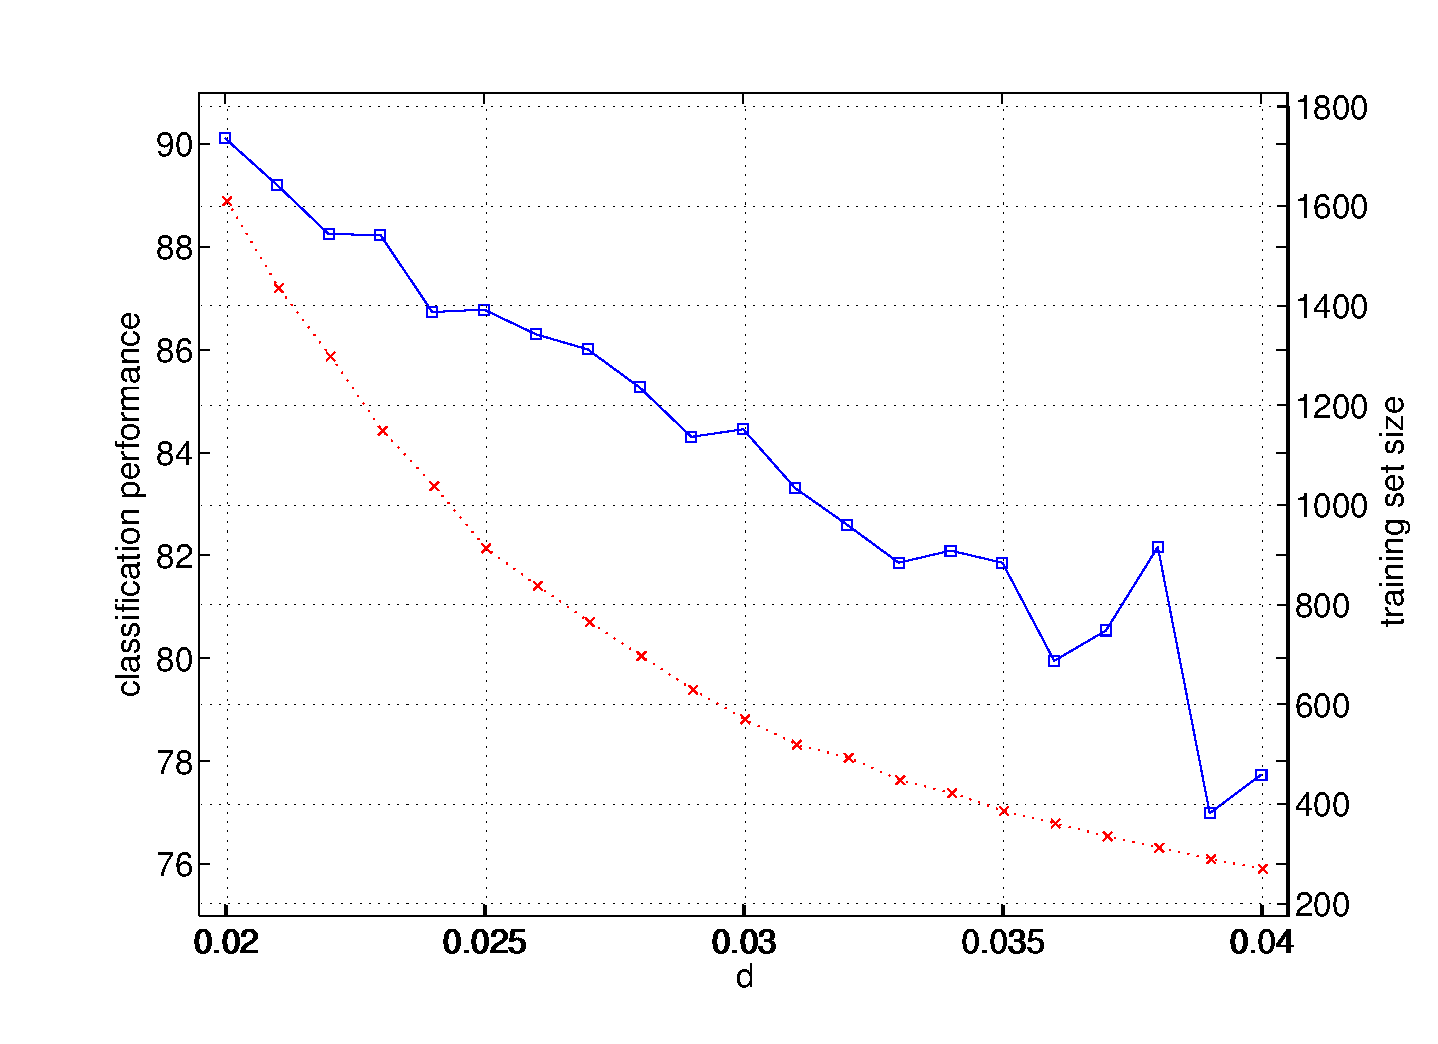
\includegraphics[width=0.6\textwidth]{figs/subj8} \\
  \end{tabular}
  \caption{size of the training set (dotted line) and classification
    performance (continuous line), of subject $8$ in the FA phase, as
    $d$ changes.}
  \label{fig:subj8}
\end{figure*}

The Figure confirms that the training set size has a decreasing
polynomial trend, while the performance changes linearly. In
particular, for $d=0.032$ the previously shown performance appears,
whereas if a larger performance is required, one can increase the
number of samples in the training set, or, which is equivalent, reduce
the agnitude of $d$. For instance, to get an accuracy of about $90\%$
$d$ must be set at $0.2$ ending up in a training set with some $1800$
samples.

\subsection{Cross-Subject Analysis}

We now turn our attention to cross-subject analysis, that is, how
accurate a model trained on a subject is, if tested on data gathered
from another subject. This problem is interesting in the sense that it
can shed light on common model features, hopefully paving the way for
building a pre-trained ``universal'' model, which could be shipped
along with the mechanical hand or prosthesis, and dramatically reduce
the human subject's training time.

Recall that in this experiment, for all subjects, the EMG electrodes
were carefully positioned on the forearm according to an anatomical
guideline, meaning that noise due to inter-arm differences should be
to some extent avoided. We can therefore check how well each model
performs on each subject by building a \emph{cross-subject performance
matrix} $A$, for both classification and regression, and for both phases,
in which $A_{ij}$ is the performance index attained by a model trained
on data gathered from subject $i$ while predicting data gathered from
subject $j$. Figure \ref{fig:cross} shows the four matrices.

\begin{figure*}[!ht] \centering
  \begin{tabular}{cc}
    \includegraphics[width=0.45\textwidth]{figs/crossClass1} & \includegraphics[width=0.45\textwidth]{figs/crossClass2} \\
    $51.69\% \pm 19.27\%$ & $54.04\% \pm 16.42\%$ \\
    \includegraphics[width=0.45\textwidth]{figs/crossRegr1} & 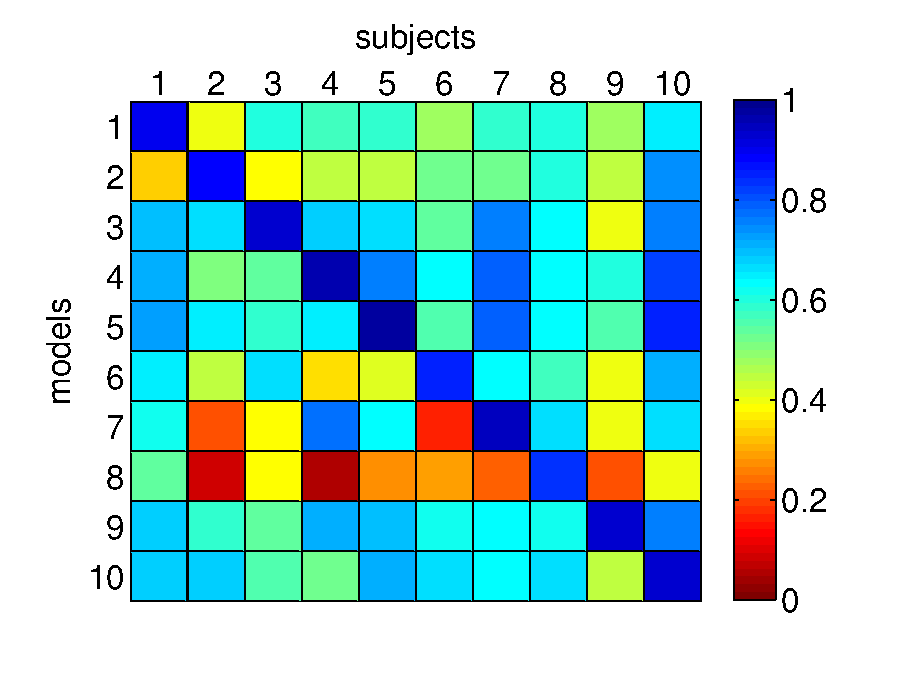
\includegraphics[width=0.45\textwidth]{figs/crossRegr2} \\
    $0.60 \pm 0.18$ & $0.58 \pm 0.19$ \\
  \end{tabular}
  \caption{cross-subject performance matrices, for classification (top
    row) and regression (bottom row), in the SA (left column)
    and FA phase (right column); the numbers refer to all element of
    the matrices, excluding the diagonals.}
  \label{fig:cross}
\end{figure*}

The overall results indicate that a large amount of the models
overlap, or at least that there is a certain cross-subject capacity of
prediction. Consider the numbers below the matrices in the Figure: in
classification, the performances are $51.69\%$ and $54.04\%$, with the
remarkable particular that the FA-models are slightly, but
consistently, \emph{better} in cross-subject analysis (higher mean
values and lower standard deviations) than the SA-models. This
indicates that, as already hinted at in the previous Subsection, the
FA-models have a wider knowledge of the respective input spaces and,
therefore, of the input space \emph{tout court}. This gives them a
little edge over the more limited SA-models.

As far as regression is concerned, things are even better, the average
cross-subject correlation being around $0.60$. To some extent, it is
likely that some of these models could actually be used as bootstrap
models for training online on new subjects. This corroborates the
hypothesis that, given a sufficiently large number of subjects, a
``common model'' could be potentially extracted, which would act as a
basis for online learning. How to build this common model is the
object of future research. Notice that, interestingly, models trained
on subjects $6$ (for the SA phase) and $8$ (FA phase) appear to be
particularly bad in predicting other subjects' data (the related rows
of the bottom left and right matrices, in turn, are rather darker than
the average).

Here the question naturally arises: what makes a model more or less
effective on ``new'' data? \footnote{this question is actually
connected to the general problem of generalisation in machine
learning; here we have no pretence of solving this problem in general,
but only to give a hint at the solution in this particular framework.}
In our previous work, we showed a significant (inverse) correlation
between the performance matrices and the \emph{cross-distance
matrices} $D$, obtained by evaluating a mean distance $D_{ij}$ between
two sample sets $S_i$ and $S_j$ like this:

$$ D_{ij} = \frac{1}{|S_j|} \sum_{s_j \in S_j}{\min_{s_i \in S_i}{ ||s_j-s_i||^2 } } $$

Here we repeat the analysis for each pair $(i,j)$ of subjects and for
the two phases and problems. The results show that inverse correlation
is absent in the case of the FA phase in classification; it is mild
($-0.32$) for SA in classification; and that it is strong in the case
of regression ($-0.63$ for the SA phase and $-0.65$ for the FA
phase). It is likely that the correlation in regression is connected
to the actual smoothness of the function the system is trying to
approximate --- a consideration which we already put forward in the
previous work. It is unclear why the classification problems show a
weak correlation or none at all.
